\documentclass[11pt, oneside]{article}   	
\usepackage[left=26mm,top=26mm,right=26mm,bottom=26mm]{geometry}    
\geometry{a4paper}                   		
\usepackage{graphicx}			
\usepackage{amssymb}
\usepackage{hyperref}
\usepackage{siunitx}
\usepackage{cite}
\usepackage{url}
\usepackage[parfill]{parskip}
\setlength{\headsep}{5pt}
\graphicspath{ {images/} }


\title{\vspace{-1.6cm}Description of the Basic System}
\author{\textit{An app for visualisation of avalanche hazard}}
\date{}							
\begin{document}
\maketitle

\section{Structure of the Visualisation System}

The application developed for this project consists of user-facing programs (represented by ovals), servers providing real-time data (represented by rectangles) and data computation programs (represented by hexagons), as shown in the followed system diagram.

\begin{figure}[h]
\centering
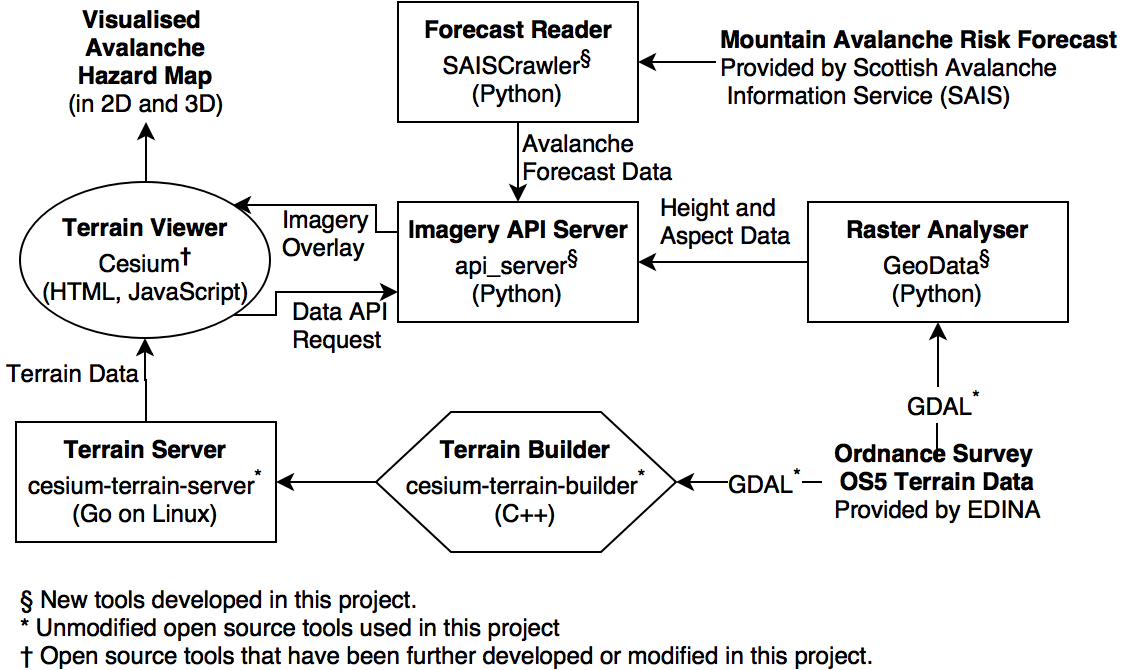
\includegraphics[scale=0.3]{System.png}
\caption{A diagram illustrating the structure of the visualisation system.}
\end{figure}

In order to properly process and visualise data from various sources to the user, several new tools have been developed to complete the tool chain, which also includes a number of existing open source tools, such as GDAL\cite{GDAL} and the Cesium Terrain Builder \cite{cesium-terrain-builder}. The data processing and visualisation processes will be covered in more detail in the next few sections.

\section{Procurement and Processing of Raster Data}
	For the basic system, height and terrain aspect data is required for geographical areas of visualisation. Although the application is developed based on the availability of avalanche risk forecasts for Scottish Highlands, with the appropriate avalanche risk forecasts and terrain raster data, this application can be trivially adapted for other mountainous areas.
	
	\subsection{Choice of Data Source}
		There are a number of available sources for Digital Elevation Model (DEM) data of the United Kingdom, most notably the EU-DEM Data \cite{eu-dem} provided by the European Commission and the UK Government's Ordnance Survey Data (OS5) \cite{os-5}, provided free for education by EDINA. 
		
		The EU-DEM Data covers the entire Western Europe with an accuracy of 25 to 30 meters, arranged in the EPSG:3035 \cite{epsg-3035} spatial reference system. The data is available in full, and can be used for both educational and commercial purposes subject to citation requirements. 
		
		The Ordnance Survey (OS5) Data covers the United Kingdom only, with a superior accuracy of 5 meters, arranged in the British National Grid \cite{osgb-1936} reference system. The data can be requested per-tile either at a cost (no usage restrictions) or free through EDINA (educational uses only), subject to citation requirements.
		
		With considerations on the nature of the project and the potential uses of the application, the Ordnance Survey Data is used for the course of the project, as an elevation model with higher accuracy is beneficial for accurate computations and evaluations. However, should an expansion of coverage or usage be required, the EU-DEM Data can be processed and used with the same procedures.
		
	\subsection{Processing of Raster Data} \label{subsec:rasterdata}
		Differing from EU-DEM, the Ordnance Survey Data is supplied on a tile-by-tile basis. Therefore to improve processing efficiency, the first part of the processing procedures is to merge the data into a single GeoTIFF \cite{geotiff} file with the GDAL tool:
		\begin{verbatim}
			find ./OS5/ -name '*.tif' | xargs gdal_merge.py -of GTiff -o OS5_Merged.tif 
		\end{verbatim}
		
		The merged DEM data is then reprojected by GDAL into the WGS84 geodetic system \cite{wgs84} that is used by the majority of mapping and navigation systems:
		\begin{verbatim}
			gdal_translate -a_srs EPSG:4326 -of GTiff OS5_Merged.tif OS5_WGS84.tif
		\end{verbatim}
		
		The reprojected elevation raster \textbf{OS5\_WGS84.tif} can now be used to look up altitude for each point in the geographical area covered by the DEM Data. However, in order to obtain a dataset of terrain aspects for each point within the same boundaries and reference system, it is also necessary to produce an aspect raster, \textbf{OS5\_WGS84\_Aspects.tif} from the elevation raster:
		\begin{verbatim}
			gdaldem aspect OS5_WGS84.tif OS5_WGS84_Aspects.tif -of GTiff
		\end{verbatim}
		
	\subsection{Retrieval of Processed Terrain Data}
		Two potential designs have been considered for the implementation of terrain data retrieval: a direct raster lookup system or a database-driven system. 
		
		A brief attempt has been made to build a key-value storage based on MongoDB\footnote{MongoDB: https://www.mongodb.com/}, with geodetic coordinates as key and taking advantage of MongoDB's geospatial system \cite{mongodb-spatial}. However, further evaluations found that although this system provides great flexibility in modifying stored data, in addition to a storage space overhead of approximately five fold, the performance of batch retrieval is insufficient for the data size involved in live operation. Therefore, this implementation has been dropped in favour of the direct raster lookup system.
		
		The direct raster lookup system (\textit{GeoData}) is built to the requirements of high-volume data retrieval, programmed with the Python bindings of the GDAL library. It operates directly on the raster files, and can read ranges of data points efficiently without the need of reading the raster into memory, due to the location-deterministic nature of the GeoTIFF format.  The data retrieval process of this system is illustrated as follows:
		\begin{figure}[h]
		\centering
		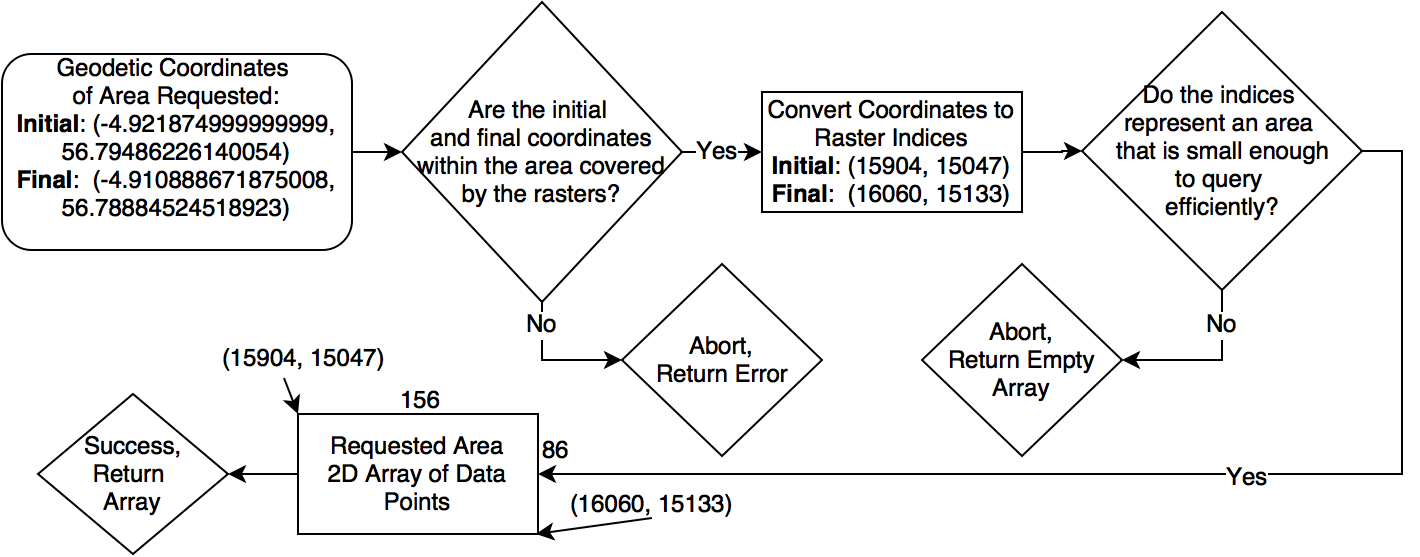
\includegraphics[scale=0.3]{Retrieval.png}
		\caption{\label{fig:retrieval}A diagram illustrating the retrieval of altitude and aspect data from their respective rasters with geodetic coordinates.}
		\end{figure}
		
		The geodetic coordinates required to retrieve the data would be supplied by the user interface through the \hyperref[sec:APIServer]{Imagery API Server}. The conversion from coordinates to raster indices is a fixed-interval sampling process, in which we have a data point for each chunk of distance equal to the resolution of the raster, which in the case of OS5 is five meters. Therefore, for the rectangular area between the two coordinates in Figure \ref{fig:retrieval}, we have a data size of 13416 ($156 \times $86).
		
\section{Procurement and Processing of Avalanche Forecast Data}
	\subsection{Retrieval of Forecast Data}
		The Scottish Avalanche Information Service (SAIS)\cite{sais} provides forecasts and information of the avalanche risks in Scottish Mountains several days a week during the winter sport season. The most prominent scale of risk is the hazard compass rose \cite[p. 4]{sais-report}, as shown in Figure \ref{fig:compassrose}. Although not completely representing the risk assessment by itself, it provides an excellent source of information in correlating altitude and aspect to the approximate level of avalanche risk, ranging from 0 (Risk Not Applicable) to 5 (Very High Risk), which can be used as part of a data model in estimating avalanche risk.
		\begin{figure}[h]
		\centering
		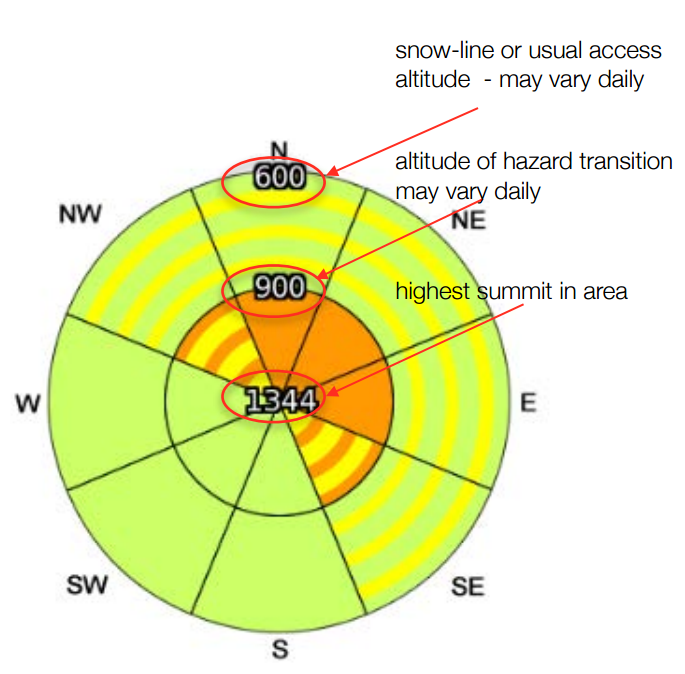
\includegraphics[scale=0.3]{CompassRose.png}
		\caption{\label{fig:compassrose}An example compass rose produced by the SAIS.\cite[p. 4]{sais-report}}
		\end{figure}
		
		Unfortunately, the SAIS does not provide an API with which the risk levels making up the compass rose could be retrieved easily. Therefore, it was necessary to build a web crawler (\textit{SAISCrawler}) with the Selenium library \footnote{Selenium: http://docs.seleniumhq.org/} to automatically search for and download avalanche forecasts from the SAIS.
		
		The crawler retrieves forecast data by visiting a predefined list of SAIS location pages, each corresponding to a location under observation, and then locate a list of forecasts conducted for that location. Each forecast has a unique page containing the image link to the compass rose for the forecast, and the URL encoding of the image link contains the altitude thresholds and risk levels that can be stored. 
		
	\subsection{Structure and Storage of Forecast Data}
	
		Vertically, the forecast data is divided by altitude into two sectors, each of which is further divided by terrain aspect into eight sections, each represents a 30\si{\degree} circular segment, as depicted in Figure \ref{fig:compassrose}. Each segment contains two risk levels: the primary level and the secondary level. Therefore, a total of 32 risk level values are extracted from each compass rose. 
		
		In conformity with the entity-relationship model, eight forecast records are created for the eight circular segments, each containing the primary and secondary risk levels for the two altitude sectors in that segment, along with the date of forecast and the transition altitudes. These records are stored in the SQLite database \footnote{SQLite: https://sqlite.org/} by the crawler. An example set of forecast records is depicted in Figure \ref{fig:sqlite}.
		
		\begin{figure}[h]
		\centering
		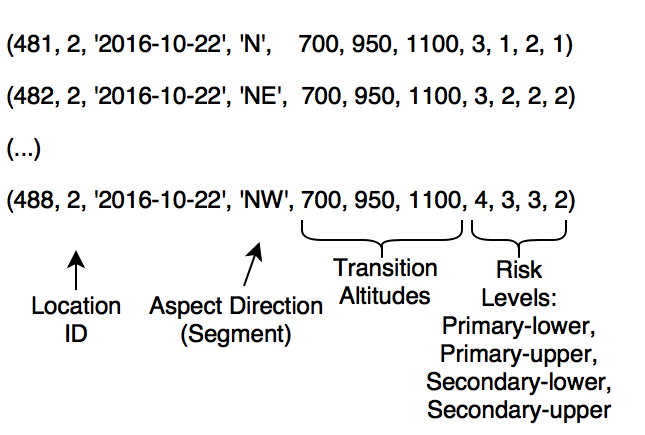
\includegraphics[scale=0.3]{SQLite.png}
		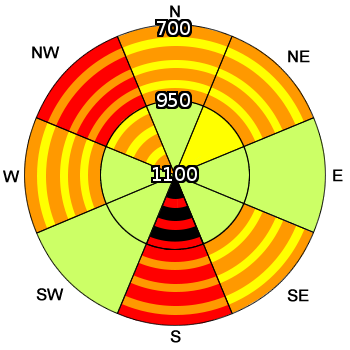
\includegraphics[scale=0.5]{DangerousRose.png}
		\caption{\label{fig:sqlite}An example set of forecast records (left) extracted from a compass rose (right) \cite{sais}.}
		\end{figure}
		
		A Python database interface for the SQLite database has been included with \textit{SAISCrawler} for the data to be retrieved by other parts of the application.

\section{Construction and Presentation of the 3D Terrain Model}

	A User Interface is necessary for presenting the visualised hazard to the user. Rather than developing a new 3D terrain viewer -- a time-consuming process which deviates from the purpose of this project -- the decision was taken to adapt the open source map engine Cesium \footnote{Cesium: https://cesiumjs.org} for this purpose.
	
	\subsection{Choice of Terrain Data Source for the 3D Model}
	
	 	The initiator of the Cesium project, Analytical Graphics, Inc, has made available the STK World Terrain Server \cite{stk-world-terrain} for public online use. Within the European Union area, the STK World Terrain uses model from the EU-DEM Data \cite{eu-dem}, therefore having a resolution of 25 to 30 meters. 
		
		Alternatively, the height map data from the Ordnance Survey OS5 \cite{os-5} can also be used to construct terrain models for displaying in Cesium, with the Cesium Terrain Builder \cite{cesium-terrain-builder} tool made by University of Southampton. The terrain model will therefore carry the improved OS5 resolution of 5 meters. However, there are a few constraints to the construction of terrain models from the large OS5 dataset, as explained in \ref{subsec:construction}.
		
	\subsection{Construction of the 3D Model} \label{subsec:construction}
		
		The 3D terrain model for Cesium is organised in the \textit{heightmap-1.0}\cite{heightmap} format. If the STK World Terrain is used, no model construction is required, as the model is directly available (and default in Cesium) from the STK World Terrain Server. 
		
		To construct a 3D terrain model from another data source, such as OS5, the Cesium Terrain Builder tool can convert a GeoTIFF raster into the \textit{heightmap-1.0} format:
		\begin{verbatim}
			ctb-tile --output-dir ./heightmap/ --start-zoom 18 --end-zoom 0 sourceRaster.tif
		\end{verbatim}
		
		However, due to the need of resampling data from the source raster, when the raster size is large, the data index can easily overflow at lower zoom levels, where the ranges of tile indices are vast.  An index overflow will trigger an error that prevents the terrain building process from completion, often after hours of computations on a high performance computer. 
		
		While determining the exact limit of the raster size is difficult, we were able to completely construct the terrain model of a 50km-by-50km area (covering each of the six forecast areas of SAIS). Six of these terrain models have been constructed for the six areas. The constructed terrain models can then be served to Cesium with the separate Cesium Terrain Server \cite{cesium-terrain-server} tool.
		
		It is however impossible to completely construct the full terrain model from a raster covering all forecast areas, such as \textbf{OS5\_WGS84.tif} generated in \ref{subsec:rasterdata}, despite our attempt to build each level separately from the Virtual Raster dataset of the level above ({\path{Scripts/build_by_level.py}), as the index would still overflow when converting from zoom level 4 to level 3.
		
	\subsection{Presentation of the 3D Model in Cesium}
		
		An HTML and JavaScript web application has been built with the Cesium library to create the user interface of the application that can be used on both desktop and mobile devices. The web application will first load a 3D terrain model from the chosen terrain source, and then request imagery overlays from our Imagery API server as described in \ref{sec:APIServer} to visualise an avalanche hazard layer on top of the terrain model, as shown in Figure \ref{fig:UI}.
		\begin{figure}[h]
		\centering
		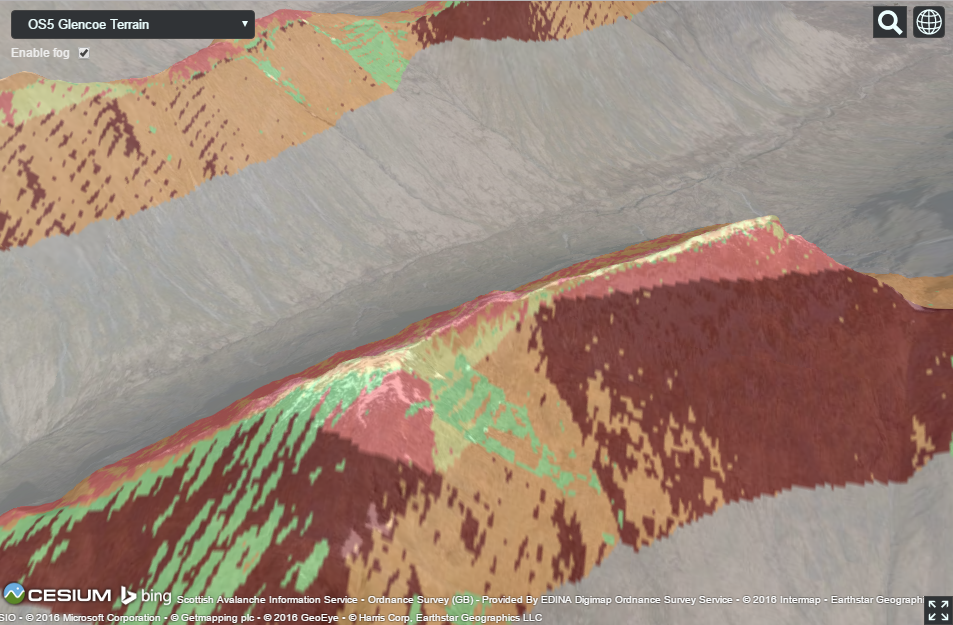
\includegraphics[scale=0.5]{UI.png}
		\caption{\label{fig:UI}The user interface of the basic system in operation.}
		\end{figure}
		
		
		As Cesium supports switching between terrain model sources without reloading the entire JavaScript terrain viewer, both our self-hosted OS5 terrain models and the model from the STK World Terrain can be loaded by the user through selecting from the drop-down menu at top left corner of the application. 
		
\section{API Interfacing of \textit{GeoData} and the User Interface} \label{sec:APIServer}
	
	
		
		
		
\bibliographystyle{IEEEtran}
\small{\bibliography{project}}
\end{document}  